\documentclass[]{book}
\usepackage{lmodern}
\usepackage{amssymb,amsmath}
\usepackage{ifxetex,ifluatex}
\usepackage{fixltx2e} % provides \textsubscript
\ifnum 0\ifxetex 1\fi\ifluatex 1\fi=0 % if pdftex
  \usepackage[T1]{fontenc}
  \usepackage[utf8]{inputenc}
\else % if luatex or xelatex
  \ifxetex
    \usepackage{mathspec}
  \else
    \usepackage{fontspec}
  \fi
  \defaultfontfeatures{Ligatures=TeX,Scale=MatchLowercase}
\fi
% use upquote if available, for straight quotes in verbatim environments
\IfFileExists{upquote.sty}{\usepackage{upquote}}{}
% use microtype if available
\IfFileExists{microtype.sty}{%
\usepackage{microtype}
\UseMicrotypeSet[protrusion]{basicmath} % disable protrusion for tt fonts
}{}
\usepackage[margin=1in]{geometry}
\usepackage{hyperref}
\hypersetup{unicode=true,
            pdftitle={Udvidet Statistik for de finansielle uddannelser.},
            pdfauthor={Thomas Petersen},
            pdfborder={0 0 0},
            breaklinks=true}
\urlstyle{same}  % don't use monospace font for urls
\usepackage{natbib}
\bibliographystyle{apalike}
\usepackage{longtable,booktabs}
\usepackage{graphicx,grffile}
\makeatletter
\def\maxwidth{\ifdim\Gin@nat@width>\linewidth\linewidth\else\Gin@nat@width\fi}
\def\maxheight{\ifdim\Gin@nat@height>\textheight\textheight\else\Gin@nat@height\fi}
\makeatother
% Scale images if necessary, so that they will not overflow the page
% margins by default, and it is still possible to overwrite the defaults
% using explicit options in \includegraphics[width, height, ...]{}
\setkeys{Gin}{width=\maxwidth,height=\maxheight,keepaspectratio}
\IfFileExists{parskip.sty}{%
\usepackage{parskip}
}{% else
\setlength{\parindent}{0pt}
\setlength{\parskip}{6pt plus 2pt minus 1pt}
}
\setlength{\emergencystretch}{3em}  % prevent overfull lines
\providecommand{\tightlist}{%
  \setlength{\itemsep}{0pt}\setlength{\parskip}{0pt}}
\setcounter{secnumdepth}{5}
% Redefines (sub)paragraphs to behave more like sections
\ifx\paragraph\undefined\else
\let\oldparagraph\paragraph
\renewcommand{\paragraph}[1]{\oldparagraph{#1}\mbox{}}
\fi
\ifx\subparagraph\undefined\else
\let\oldsubparagraph\subparagraph
\renewcommand{\subparagraph}[1]{\oldsubparagraph{#1}\mbox{}}
\fi

%%% Use protect on footnotes to avoid problems with footnotes in titles
\let\rmarkdownfootnote\footnote%
\def\footnote{\protect\rmarkdownfootnote}

%%% Change title format to be more compact
\usepackage{titling}

% Create subtitle command for use in maketitle
\newcommand{\subtitle}[1]{
  \posttitle{
    \begin{center}\large#1\end{center}
    }
}

\setlength{\droptitle}{-2em}

  \title{Udvidet Statistik for de finansielle uddannelser.}
    \pretitle{\vspace{\droptitle}\centering\huge}
  \posttitle{\par}
    \author{Thomas Petersen}
    \preauthor{\centering\large\emph}
  \postauthor{\par}
      \predate{\centering\large\emph}
  \postdate{\par}
    \date{2018-07-28}

\usepackage{booktabs}
\usepackage{amsthm}
\makeatletter
\def\thm@space@setup{%
  \thm@preskip=8pt plus 2pt minus 4pt
  \thm@postskip=\thm@preskip
}
\makeatother

\begin{document}
\maketitle

{
\setcounter{tocdepth}{1}
\tableofcontents
}
\hypertarget{matematik-med-konomisk-profil.}{%
\chapter*{Matematik med økonomisk
profil.}\label{matematik-med-konomisk-profil.}}
\addcontentsline{toc}{chapter}{Matematik med økonomisk profil.}

\hypertarget{Settings}{}

\hypertarget{TopBar}{}
\hypertarget{Sentry_label}{}
\protect\hypertarget{Sentry_label_span}{}{Login eller opret klik her}

\hypertarget{magicGroup}{}
\hypertarget{messages}{}
.

\hypertarget{Sentry_emailDiv}{}
{ }

\hypertarget{Sentry_passwordDiv}{}
{ }

\hypertarget{Sentry_HIDpasswordDiv}{}
{ }

\hypertarget{unHideDiv}{}
\protect\hypertarget{forgotSpan}{}{Glemt?}
\protect\hypertarget{unHideSpan}{}{Vis}

\hypertarget{buttonDiv}{}
klik

\hypertarget{psistDiv}{}
 \protect\hypertarget{psistSpan}{}{Husk mig}

\hypertarget{goInside}{}
\protect\hypertarget{goInsideSpan}{}{.}

\hypertarget{myProfile}{}
Min profil

\hypertarget{Tilmeld}{}
Opret

\hypertarget{logOut}{}
{Log Out}

\hypertarget{xbox}{}

\hypertarget{Sentry_noJSLogin}{}
{Javascript Required}

\hypertarget{Sentry_loggingIn}{}

\hypertarget{Sentry_In}{}
For testing.

You must have JavaScript enabled in order to log in.

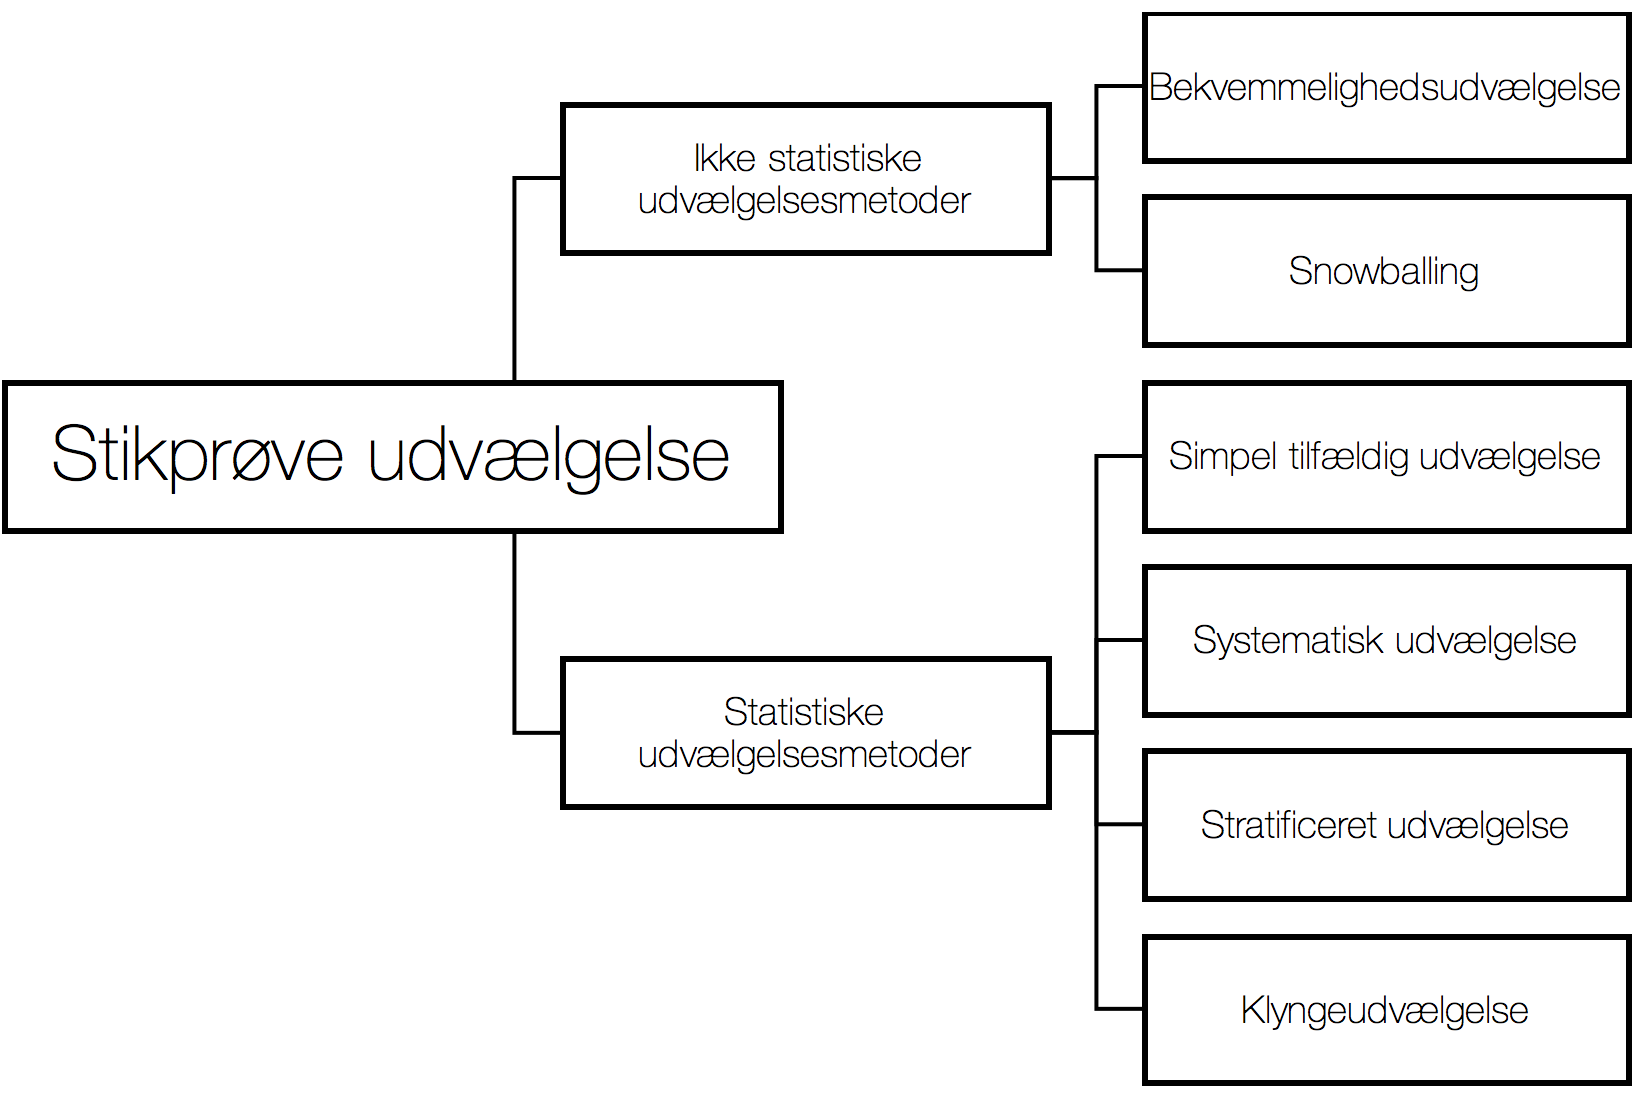
\includegraphics[width=6.37083in,height=0.75278in]{media/image1.png}\includegraphics[width=6in,height=0.68926in]{media/image2.emf}\includegraphics[width=8.5in,height=12.69722in]{media/image3.jpg}

\hypertarget{table-of-contents}{%
\chapter{Table of Contents}\label{table-of-contents}}

\protect\hyperlink{indledning}{{[}2{]} {[}Indledning{]} 3}

{[}{[}3{]}
\protect\hyperlink{grundluxe6ggende-regneregler}{Grundlæggende
regneregler}

{[}{[}3.1{]} \protect\hyperlink{reduktions-regneregler}{Reduktions
regneregler}

{[}{[}3.2{]} \protect\hyperlink{bruxf8kregneregler}{Brøkregneregler}

{[}{[}3.3{]} \protect\hyperlink{procentregneregler}{Procentregneregler}

{[}{[}3.4{]} \protect\hyperlink{indekstal}{Indekstal}

{[}{[}3.5{]} \protect\hyperlink{procentpoint}{Procentpoint}

{[}{[}3.6{]} \protect\hyperlink{potensregneregler}{Potensregneregler}

{[}{[}4{]} \protect\hyperlink{lineuxe6re-funktioner}{Lineære funktioner}

{[}{[}4.1{]} \protect\hyperlink{generel-forskift}{Generel Forskift}

{[}{[}4.2{]}
\protect\hyperlink{bestemmelse-af-forskrift-baseret-puxe5-2-punkter}{Bestemmelse
af forskrift baseret på 2 punkter}

{[}{[}4.3{]} \protect\hyperlink{luxf8sning-af-ligninger}{Løsning af
ligninger}

{[}{[}4.4{]} \protect\hyperlink{ligninger-med-2-ubekendte.}{2 ligninger
med 2 ubekendte.}

{[}{[}4.5{]}
\protect\hyperlink{udbuds--og-efterspuxf8rgselskurver}{Udbuds- og
efterspørgselskurver}

{[}{[}4.6{]}
\protect\hyperlink{addition-af-lineuxe6re-funktioner}{Addition af
lineære funktioner}

{[}{[}4.6.1{]}
\protect\hyperlink{vertikal-addition-af-lineuxe6re-funktioner}{Vertikal
addition af lineære funktioner}

{[}{[}4.6.2{]}
\protect\hyperlink{horisontal-addition-af-lineuxe6re-funktioner}{Horisontal
addition af lineære funktioner}

{[}{[}4.7{]} \protect\hyperlink{priselasticitet}{Priselasticitet}

{[}{[}4.7.1{]} \protect\hyperlink{video-om-priselasticitet}{Video om
priselasticitet}

{[}{[}5{]} \protect\hyperlink{polynomier}{Polynomier}

{[}{[}5.1{]} \protect\hyperlink{gradspolynomier}{2. Gradspolynomier}

{[}{[}5.1.1{]} \protect\hyperlink{video-2.-gradspolynomier}{Video 2.
Gradspolynomier}

{[}{[}6{]} \protect\hyperlink{eksponentielle-funktioner}{Eksponentielle
funktioner}

{[}{[}6.1{]}
\protect\hyperlink{fordoblings--og-halveringskonstant.}{Fordoblings- og
halveringskonstant.}

{[}{[}7{]} \protect\hyperlink{finansiel-regning}{Finansiel regning}

{[}{[}7.1.1{]}
\protect\hyperlink{nutidsvuxe6rdi-og-fremtidsvuxe6rdi-af-en-kapital}{Nutidsværdi
og fremtidsværdi af en kapital}

{[}{[}7.2{]} \protect\hyperlink{annuiteter}{Annuiteter}

{[}{[}7.2.1{]}
\protect\hyperlink{fremtidsvuxe6rdi-af-en-annuitet}{Fremtidsværdi af en
annuitet}

\protect\hyperlink{nutidsvuxe6rdi-af-en-annuitet}{{[}7.2.2{]}
{[}Nutidsværdi af en annuitet{]} 49}

\protect\hyperlink{inverse-funktioner}{{[}8{]} {[}Inverse funktioner{]}
52}

\protect\hyperlink{logaritmefunktioner}{{[}9{]}
{[}Logaritmefunktioner{]} 54}

\protect\hyperlink{differentialregning}{{[}10{]}
{[}Differentialregning{]} 58}

\protect\hyperlink{regneregler-differentiation}{{[}10.1{]}
{[}Regneregler differentiation{]} 60}

\protect\hyperlink{differentiation-af-sammensatte-funktioner.}{{[}10.2{]}
{[}Differentiation af sammensatte funktioner.{]} 61}

\protect\hyperlink{ekstremumspunkter}{{[}10.3{]} {[}Ekstremumspunkter{]}
62}

\protect\hyperlink{lokale-og-globale-ekstremumspunkter}{{[}10.4{]}
{[}Lokale og globale ekstremumspunkter{]} 64}

\protect\hyperlink{konveksitet-og-konkavitet}{{[}10.5{]} {[}Konveksitet
og konkavitet{]} 65}

\protect\hyperlink{sammenhuxe6nge-avc-atc-tc-tr-mc-mr-og-mathbfpi}{{[}10.6{]}
{[}Sammenhænge AVC, ATC, TC, TR, MC, MR og{]} 66}

\protect\hyperlink{optimeringseksempel}{{[}10.7{]}
{[}Optimeringseksempel{]} 68}

\protect\hyperlink{partielle-afledede-og-gradienten}{{[}11{]}
{[}Partielle afledede og gradienten{]} 72}

\protect\hyperlink{video-om-partielle-afledede-og-gradienten}{{[}11.1.1{]}
{[}Video om partielle afledede og gradienten{]} 72}

\protect\hyperlink{cobb-douglas-funktioner}{{[}11.2{]} {[}Cobb-Douglas
funktioner{]} 77}

\protect\hyperlink{video-produktionsfunktioner}{{[}11.2.1{]} {[}Video
produktionsfunktioner{]} 77}

\protect\hyperlink{isoquantisokvant-kurver}{{[}11.3{]}
{[}Isoquant/isokvant kurver{]} 80}

\protect\hyperlink{isocostisokost-kurver}{{[}11.4{]} {[}Isocost/Isokost
kurver{]} 83}

\protect\hyperlink{video-isocost-kurver}{{[}11.4.1{]} {[}Video isocost
kurver{]} 83}

\protect\hyperlink{eksempel-puxe5-optimering-af-produktionsoutput-for-fast-omkostningsniveau}{{[}11.4.3{]}
{[}Eksempel på optimering af produktionsoutput for fast
omkostningsniveau{]} 86}

\protect\hyperlink{video-optimering-af-produktionsoutput-for-fast-omkostningsniveau}{{[}11.4.4{]}
{[}Video optimering af produktionsoutput for fast omkostningsniveau{]}
86}

\protect\hyperlink{eksempel-puxe5-optimering-af-omkostningsniveauet-for-fast-produktionsniveau}{{[}11.4.5{]}
{[}Eksempel på optimering af omkostningsniveauet for fast
produktionsniveau{]} 89}

\protect\hyperlink{integralregning}{{[}12{]} {[}Integralregning{]} 93}

\protect\hyperlink{partiel-integration}{{[}12.1{]} {[}Partiel
integration{]} 94}

\protect\hyperlink{arealberegning}{{[}12.2{]} {[}Arealberegning{]} 94}

\protect\hyperlink{excel-simpel-brug}{{[}13{]} {[}Excel simpel brug{]}
96}

\protect\hyperlink{video-excel-simpel-brug}{{[}13.1.1{]} {[}Video excel
simpel brug{]} 96}

\protect\hyperlink{excel-investering}{{[}14{]} {[}Excel Investering{]}
103}

\protect\hyperlink{video-om-investering-med-excel}{{[}14.1.1{]} {[}Video
om investering med excel{]} 103}

\protect\hyperlink{investeringer-med-ikke-periodiske-varierende-betalingsstruxf8mme-i-excel}{{[}14.2{]}
{[}Investeringer med ikke-periodiske varierende betalingsstrømme i
excel{]} 104}

\protect\hyperlink{excel-muxe5lsuxf8gning}{{[}15{]} {[}Excel
målsøgning{]} 105}

\protect\hyperlink{excel-lineuxe6r-programmering}{{[}16{]} {[}Excel
lineær programmering{]} 107}

\protect\hyperlink{excel-lineuxe6r-regression}{{[}17{]} {[}Excel Lineær
regression{]} 114}

\protect\hyperlink{video-excel-lineuxe6r-regression}{{[}17.1.1{]}
{[}Video excel lineær regression{]} 114}

{[}{[}17.1.2{]} \protect\hyperlink{video-jmp-regressionseksempel}{Video
JMP regressionseksempel}

{[}{[}18{]}
\protect\hyperlink{luxf8sning-af-ligningssystemer-med-excel}{Løsning af
ligningssystemer med excel}

{[}{[}19{]} \protect\hyperlink{excel-omkostnings-eksempel}{Excel
omkostnings-eksempel}

{[}{[}20{]} \protect\hyperlink{excel-oversuxe6ttelser}{Excel
oversættelser}

\hypertarget{indledning}{%
\chapter{Indledning}\label{indledning}}

Noterne her omhandler matematik, man som økonom vil få brug for under
sit studie. Der findes en del bøger og videoer, der kan være til
yderligere hjælp.

Man gratis hente Troels Troelsen's bog og andre matematik og
statistikbøger på bookboon:

\href{http://bookboon.com/dk/grundlaeggende-matematik-for-oekonomer-ebook\#download}{{[}``Grundlæggende
Matematik for økonomer''{]}}

Jeg har selv lavet nogle video screencasts om diverse emner indenfor
matematik og statistik de findes på:

\href{http://www.youtube.com/ThomasPetersenMat}{{[}http://www.youtube.com/ThomasPetersenMat{]}}

Der er en matematik kanal på youtube, med mange gode videoer fra
ingeniøren

\href{http://www.youtube.com/user/matematikkanalen}{{[}http://www.youtube.com/user/matematikkanalen{]}}

Der er en god hjemmeside med mange danske gratis matematikvideoer:

\href{http://www.frividen.dk/default.aspx}{{[}http://www.frividen.dk/default.aspx{]}}

En HA-studerende har lavet en hjemmeside med excel kursus.

\href{http://www.excelkursus.com/}{{[}www.excelkursus.com{]}}

Jeg også anbefale Kahn Akademy's matematikvideoer, disse videoer er på
engelsk.

\href{http://www.youtube.com/user/khanacademy}{{[}http://www.youtube.com/user/khanacademy{]}}

Ofte vil de man kunne finde gode videoer på engelsk på Youtube om de
lidt sværere emner.

Jeg kan anbefale at man benytter f.eks.
\href{http://www.wolframalpha.com/}{{[}http://www.wolframalpha.com/{]}}
som facitliste når man løser opgaver.

\hypertarget{grundlggende-regneregler}{%
\chapter{Grundlæggende regneregler}\label{grundlggende-regneregler}}

\hypertarget{reduktions-regneregler}{%
\section{Reduktions regneregler}\label{reduktions-regneregler}}

Når a, b og c d er reelle tal gælder:

\(a + b = b + a\)

\[2 + 4 = 4 + 2\]

\(a + (b + c) = (a + b) + c = a + b + \text{c\ }\)

\[3 + \left( 4 + 5 \right) = \left( 3 + 4 \right) + 5 = 3 + 4 + 5 = 12\]

\[a + \left( b + c - d \right) = a + b + c - \text{d\ }\]

\[3 + \left( 4 + 5 - 6 \right) = 3 + 4 + 5 - 6 = 6\]

\(a - \left( b + c - d \right) = a - b - c + \text{d\ }\)

\(3 - \left( 4 + 5 - 6 \right) = 3 - 4 - 5 + 6 = 0\)

Husk reglen om at ændre fortegn på alle led når man hæver en negativ
parentes.

\[a \cdot b\  = b \cdot a\ \]

\hypertarget{cdot-4-4-cdot-3-12}{%
\section{\texorpdfstring{\[3 \cdot 4 = 4 \cdot 3 = 12\]}{3 \textbackslash{}cdot 4 = 4 \textbackslash{}cdot 3 = 12}}\label{cdot-4-4-cdot-3-12}}

\[a \cdot \left( b \cdot c \right) = \left( a \cdot b \right) \cdot c\  = a \cdot b \cdot c\ \]

\[3 \cdot \left( 4 \cdot 5 \right) = \left( 3 \cdot 4 \right) \cdot 5 = 3 \cdot 4 \cdot 5 = 60\]

\[a \cdot \left( b + c \right) = a \cdot b + a \cdot c\ \]

\[3 \cdot \left( 4 + 5 \right) = 3 \cdot 4 + 3 \cdot 5 = 27\]

Bemærk faktoren skal ganges på alle led i parentesen

\[a \cdot \left( b - c \right) = a \cdot b - a \cdot c\ \]

\[3 \cdot \left( 4 - 5 \right) = 3 \cdot 4 - 3 \cdot 5 = - 3\]

\(\left( a + b \right) \cdot \left( c + d \right) = a \cdot \left( c + d \right) + b \cdot (c + d) = a \cdot c + a \cdot d + b \cdot c + b \cdot d\\)

\(\left( 3 + 4 \right) \cdot \left( 5 + 6 \right) = 3 \cdot 5 + 3 \cdot 6 + 4 \cdot 5 + 4 \cdot 6\)

\(\left( a + b \right)^{2} = \left( a + b \right) \cdot \left( a + b \right) = a^{2} + b^{2} + 2ab\)

\[\left( 2x + 3y \right)^{2} = 4x^{2} + 9y^{2} + 12xy\]

Kvadratet af en toleddet størrelse, er kvadratet på første led +
kvadratet på andet led plus det dobbelte produkt

\(\left( a - b \right)^{2} = \left( a - b \right) \cdot \left( a - b \right) = a^{2} + b^{2} - 2ab\)

\[\left( 2x + 3y \right)^{2} = 4x^{2} + 9y^{2} + 12xy\]

Kvadratet af en toleddet størrelse, er kvadratet på første led +
kvadratet på andet led minus det dobbelte produkt

\(\left( a + b \right) \cdot \left( a - b \right) = a^{2} - b^{2}\)

\[\left( 2x + 3y \right) \cdot \left( 2x - 3y \right) = 4x^{2} - 9y^{2}\]

\hypertarget{brkregneregler}{%
\section{Brøkregneregler}\label{brkregneregler}}

En brøk består af en tæller øverst og en nævner nederst\(.\) Hvis man
tænker på tælleren som hvor mange stykker lagkage der er, og nævneren
som hvor store stykkerne er. En brøk repræsenterer det præcise tal man
får ved at dividere tælleren med nævneren. \(\frac{1}{3}\)repræsenterer
således \(1:3\), der udtrykt
som~\href{https://da.wikipedia.org/w/index.php?title=Decimalbr\%C3\%B8k\&action=edit\&redlink=1}{decimalbrøk}~er
ca. 0,6667, dette tal kan faktisk ikke skrives helt præcist som
et~\href{https://da.wikipedia.org/wiki/Decimaltal}{decimaltal}, så
brøker er fine hvis man ønsker at beregne noget helt eksakt. Der gælder
at hvis både tæller og nævner er
et~\href{https://da.wikipedia.org/wiki/Heltal}{heltal} \(\mathbb{Z}\),
så er brøken
et~\href{https://da.wikipedia.org/wiki/Rationale_tal}{rationalt tal}.

Man kan forlænge brøker ved at gange med samme tal i tæller og nævner:

\[\frac{a}{b} = \frac{a \cdot c}{b \cdot c}\]

Man kan forkorte brøker ved at dividere med samme tal i tæller og
nævner, det er god stil når man rapporterer et brøktal som slutresultat,
at dette er mest muligt forkortet:

\[\frac{a}{b} = \frac{\frac{a}{c}}{\frac{b}{c}}\]

Hvis 2 brøker har samme nævner kan man addere eller subtrahere dem
direkte.

\[\frac{a}{c} + \frac{b}{c} = \frac{a + b}{c}\]

\[\frac{a}{c} - \frac{b}{c} = \frac{a - b}{c}\]

Har 2 brøker ikke samme nævner, må man først skaffe fællesnævner ved at
forlænge den ene eller begge. Er man i tvivl kan man altid forlænge
begge brøker, med den anden brøks nævner således er man sikker på at de
har fællesnævner.

\[\frac{a}{c} + \frac{b}{d} = \frac{a \cdot d}{c \cdot d} + \frac{b \cdot c}{c \cdot d} = \frac{a \cdot d + b \cdot c}{c \cdot d}\]

\[\frac{a}{c} - \frac{b}{d} = \frac{a \cdot d}{c \cdot d} - \frac{b \cdot c}{c \cdot d} = \frac{a \cdot d - b \cdot c}{c \cdot d}\]

Man ganger en brøk med et tal, ved at gange tallet med tælleren.

\[\frac{a}{b} \cdot c = \frac{a \cdot c}{b}\]

Brøk gange brøk er tæller gange tæller og nævner gange nævner.

\[\frac{a}{b} \cdot \frac{c}{d} = \frac{a \cdot c}{b \cdot d}\]

Man dividerer en brøk med et tal, ved at gange tallet ind i nævneren.

\[\frac{a}{b}:c = \frac{a}{b \cdot c}\]

Man dividerer et tal med en brøk, ved at gange tallet med den omvendte
brøk.

\[c:\frac{a}{b} = \frac{c \cdot b}{a}\]

Man dividerer en brøk med en anden, ved at gange den første med den
omvendte brøk.

\[\frac{a}{b}:\frac{c}{d} = \frac{a \cdot d}{b \cdot c}\]

\bibliography{book.bib,packages.bib}


\end{document}
